\documentclass[a4paper,12pt]{article}
\usepackage{amsmath}
\usepackage{hyperref}
 \usepackage{graphicx}
 \usepackage{float}
 \usepackage{subcaption}
 \usepackage{listings}
 \usepackage{circuitikz}
\title{Lab Report1}
\author{Arnav Yadnopavit- EE24BTECH11007\\Prajwal - EE24BTECH11051}
\date{\today}

\begin{document}

\maketitle
\section*{Objective}
To analyze the magnitude and phase response of 1-stage, 2-stage, and 3-stage RC low-pass filters using Bode plots.

\section*{Apparatus}
\begin{itemize}
    \item Resistors (1$k\Omega$ each)
    \item Capacitors (100nF each)
    \item Function generator
    \item Oscilloscope
\end{itemize}

\section*{Theory}
A low-pass filter allows low-frequency signals to pass while attenuating higher-frequency signals. The transfer function for an $n$-stage RC low-pass filter is given by:
\begin{equation}
H_n(s) =\frac{V_C(s)}{V_0(s)}= \frac{1}{(1 + RCs)^n}
\end{equation}
where $R$ is the resistance and $C$ is the capacitance.

The magnitude response in dB is:
\begin{equation}
|H_n(j\omega)|_{dB} = 20n \log_{10}\left(\frac{1}{\sqrt{1+(\omega RC)^2}}\right)
\end{equation}

The phase response is:
\begin{equation}
\angle H_n(j\omega) = -n \tan^{-1}(\omega RC)
\end{equation}
\begin{figure}[H]
    \centering
    \begin{subfigure}{0.5\textwidth}
        
\begin{circuitikz}
\tikzstyle{every node}=[font=\large]

\draw (12.75,11.25) node[op amp,scale=1, yscale=-1 ] (opamp2) {};
\draw (opamp2.+) to[short] (11.25,11.75);
\draw  (opamp2.-) to[short] (11.25,10.75);
\draw (13.95,11.25) to[short](14.25,11.25);
\draw (11.25,11.75) to (10.75,11.75) node[ground]{};
\draw (8.25,9.25) to[R] (10.25,9.25);
\draw (9.25,7.5) to[R] (11.25,7.5);
\draw (11.25,7.5) to[short] (11.25,10.75);
\draw (10.25,9.25) to[short] (11.25,9.25);
\draw (8,7.5) to[sinusoidal voltage source, sources/symbol/rotate=auto] (9.25,7.5);
\draw (6.75,9.25) to[sinusoidal voltage source, sources/symbol/rotate=auto] (8.25,9.25);
\draw (11.25,9.25) to[R] (13.25,9.25);
\draw (13.25,9.25) to[short] (13.75,9.25);
\draw (13.75,9.25) to[short] (13.75,11.25);
\node at (11.25,9.25) [circ] {};
\node at (13.75,11.25) [circ] {};
\draw (12.75,11.25) node[op amp,scale=1, yscale=-1 ] (opamp2) {};
\draw (opamp2.+) to[short] (11.25,11.75);
\draw  (opamp2.-) to[short] (11.25,10.75);
\draw (13.95,11.25) to[short](14.25,11.25);
\draw (6.75,9.25) to (6.75,8.75) node[ground]{};
\draw (8,7.5) to (8,7) node[ground]{};
\draw (14.25,11.25) to[short, -o] (16.25,11.25) ;
\node [font=\large] at (6.75,10.25) {$V_1$};
\node [font=\large] at (8.25,8.25) {$V_2$};
\node [font=\large] at (9.25,10) {$R_1$};
\node [font=\large] at (10.25,8.25) {$R_2$};
\node [font=\large] at (12.25,9.75) {$R_f$};
\node [font=\large] at (16,11.75) {$V_{out}$};
\end{circuitikz}
    \end{subfigure}%
    \begin{subfigure}{0.5\textwidth}
        \centering
        
\begin{circuitikz}
\tikzstyle{every node}=[font=\large]

\draw (12.75,11.25) node[op amp,scale=1, yscale=-1 ] (opamp2) {};
\draw (opamp2.+) to[short] (11.25,11.75);
\draw  (opamp2.-) to[short] (11.25,10.75);
\draw (13.95,11.25) to[short](14.25,11.25);
\draw (11.25,11.75) to (10.75,11.75) node[ground]{};
\draw (8.25,9.25) to[R] (10.25,9.25);
\draw (9.25,7.5) to[R] (11.25,7.5);
\draw (11.25,7.5) to[short] (11.25,10.75);
\draw (10.25,9.25) to[short] (11.25,9.25);
\draw (8,7.5) to[sinusoidal voltage source, sources/symbol/rotate=auto] (9.25,7.5);
\draw (6.75,9.25) to[sinusoidal voltage source, sources/symbol/rotate=auto] (8.25,9.25);
\draw (11.25,9.25) to[R] (13.25,9.25);
\draw (13.25,9.25) to[short] (13.75,9.25);
\draw (13.75,9.25) to[short] (13.75,11.25);
\node at (11.25,9.25) [circ] {};
\node at (13.75,11.25) [circ] {};
\draw (12.75,11.25) node[op amp,scale=1, yscale=-1 ] (opamp2) {};
\draw (opamp2.+) to[short] (11.25,11.75);
\draw  (opamp2.-) to[short] (11.25,10.75);
\draw (13.95,11.25) to[short](14.25,11.25);
\draw (6.75,9.25) to (6.75,8.75) node[ground]{};
\draw (8,7.5) to (8,7) node[ground]{};
\draw (14.25,11.25) to[short, -o] (16.25,11.25) ;
\node [font=\large] at (6.75,10.25) {$V_1$};
\node [font=\large] at (8.25,8.25) {$V_2$};
\node [font=\large] at (9.25,10) {$R_1$};
\node [font=\large] at (10.25,8.25) {$R_2$};
\node [font=\large] at (12.25,9.75) {$R_f$};
\node [font=\large] at (16,11.75) {$V_{out}$};
\end{circuitikz}
    \end{subfigure}
    \begin{subfigure}{0.5\textwidth}
        \centering
        
\begin{circuitikz}
\tikzstyle{every node}=[font=\large]

\draw (12.75,11.25) node[op amp,scale=1, yscale=-1 ] (opamp2) {};
\draw (opamp2.+) to[short] (11.25,11.75);
\draw  (opamp2.-) to[short] (11.25,10.75);
\draw (13.95,11.25) to[short](14.25,11.25);
\draw (11.25,11.75) to (10.75,11.75) node[ground]{};
\draw (8.25,9.25) to[R] (10.25,9.25);
\draw (9.25,7.5) to[R] (11.25,7.5);
\draw (11.25,7.5) to[short] (11.25,10.75);
\draw (10.25,9.25) to[short] (11.25,9.25);
\draw (8,7.5) to[sinusoidal voltage source, sources/symbol/rotate=auto] (9.25,7.5);
\draw (6.75,9.25) to[sinusoidal voltage source, sources/symbol/rotate=auto] (8.25,9.25);
\draw (11.25,9.25) to[R] (13.25,9.25);
\draw (13.25,9.25) to[short] (13.75,9.25);
\draw (13.75,9.25) to[short] (13.75,11.25);
\node at (11.25,9.25) [circ] {};
\node at (13.75,11.25) [circ] {};
\draw (12.75,11.25) node[op amp,scale=1, yscale=-1 ] (opamp2) {};
\draw (opamp2.+) to[short] (11.25,11.75);
\draw  (opamp2.-) to[short] (11.25,10.75);
\draw (13.95,11.25) to[short](14.25,11.25);
\draw (6.75,9.25) to (6.75,8.75) node[ground]{};
\draw (8,7.5) to (8,7) node[ground]{};
\draw (14.25,11.25) to[short, -o] (16.25,11.25) ;
\node [font=\large] at (6.75,10.25) {$V_1$};
\node [font=\large] at (8.25,8.25) {$V_2$};
\node [font=\large] at (9.25,10) {$R_1$};
\node [font=\large] at (10.25,8.25) {$R_2$};
\node [font=\large] at (12.25,9.75) {$R_f$};
\node [font=\large] at (16,11.75) {$V_{out}$};
\end{circuitikz}
    \end{subfigure}
\end{figure}
\section*{Procedure}
\begin{enumerate}
    \item Assemble the RC low-pass filter circuits for 1-stage, 2-stage, and 3-stage configurations.
    \item Apply an AC signal of varying frequency using the function generator.
    \item Measure the output voltage using the oscilloscope.
    \item Compute the magnitude and phase response.
    \item Plot the Bode magnitude and phase graphs.
\end{enumerate}
%#array([  0,-0.81643989,-28.54232711,0.,-8.31030888, -57.64807176,0.,-17.35001135,-59.13023121])
%#array([  0.  ,  25.92,  77.76,  14.4 ,  60.48, 138.24,  14.4 ,  86.4 ,169.2 ])
\section*{Readings}
\subsection*{Stage1}
\begin{figure}[H]
    \centering
    \begin{subfigure}{0.5\textwidth}
        \centering
        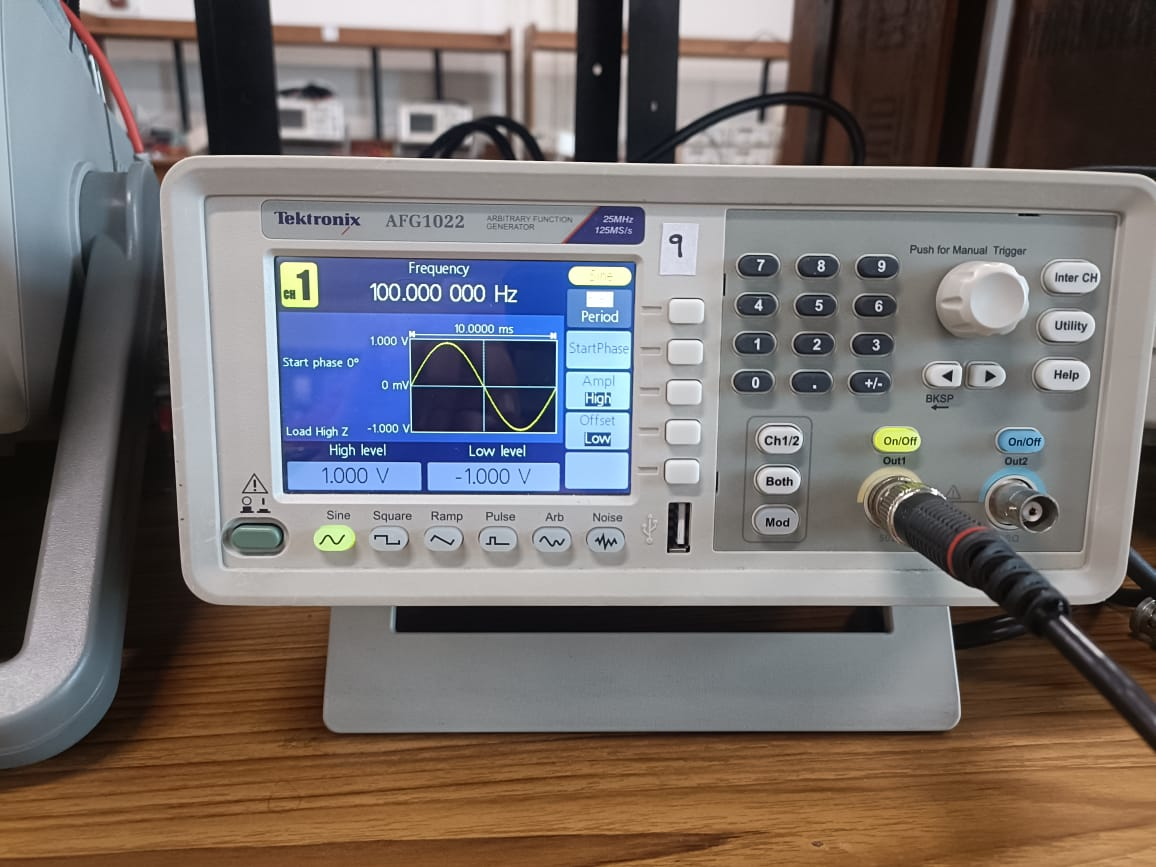
\includegraphics[height=5cm]{figs/Stage1/100/para.jpeg}
    \end{subfigure}%
    \begin{subfigure}{0.5\textwidth}
        \centering
        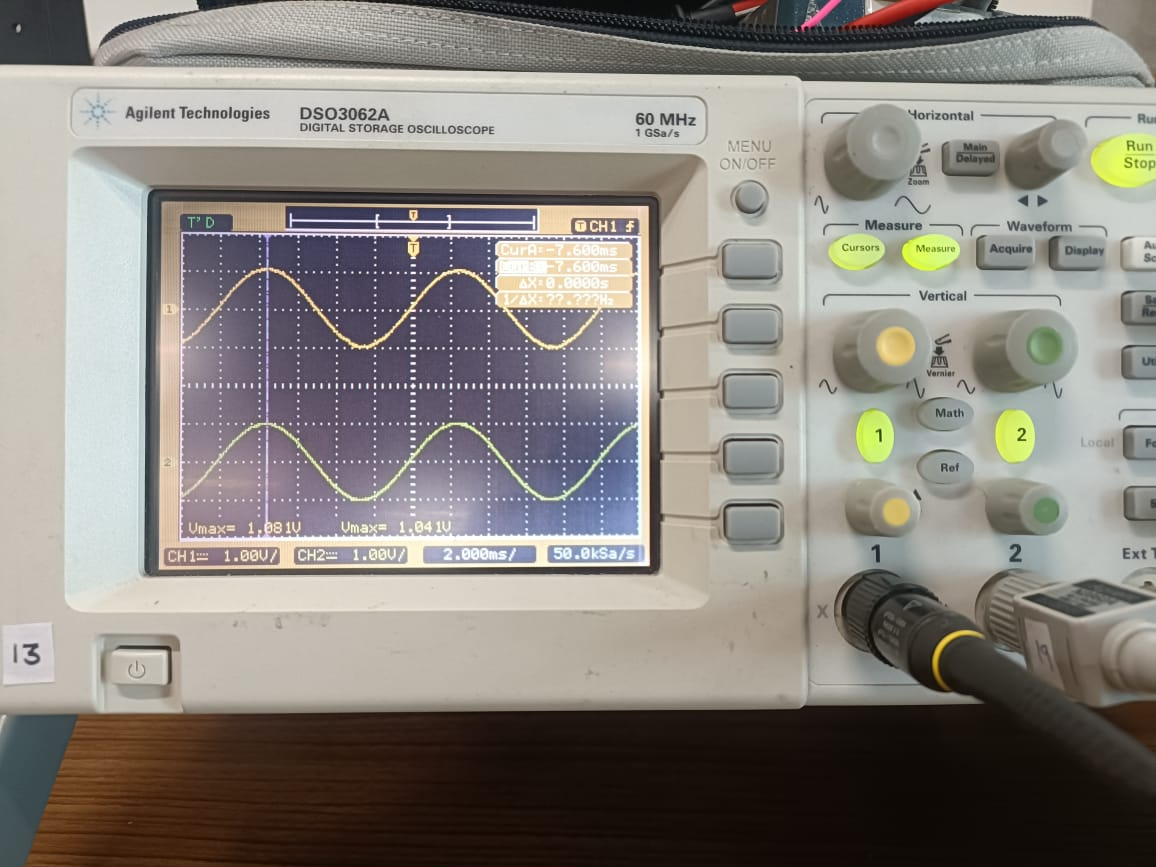
\includegraphics[height=5cm]{figs/Stage1/100/plot.jpeg}
    \end{subfigure}
\end{figure}
\begin{figure}[H]
    \centering
    \begin{subfigure}{0.5\textwidth}
        \centering
        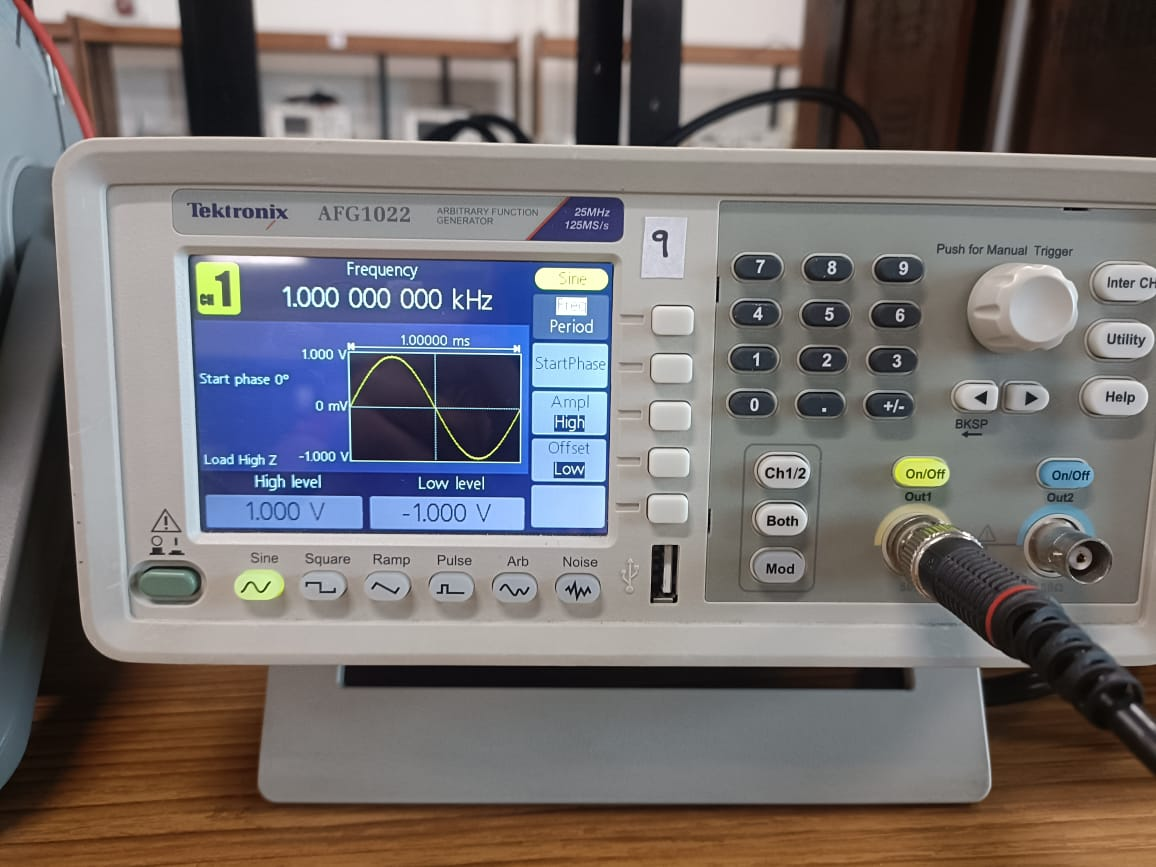
\includegraphics[height=5cm]{figs/Stage1/1000/para.jpeg}
    \end{subfigure}%
    \begin{subfigure}{0.5\textwidth}
        \centering
        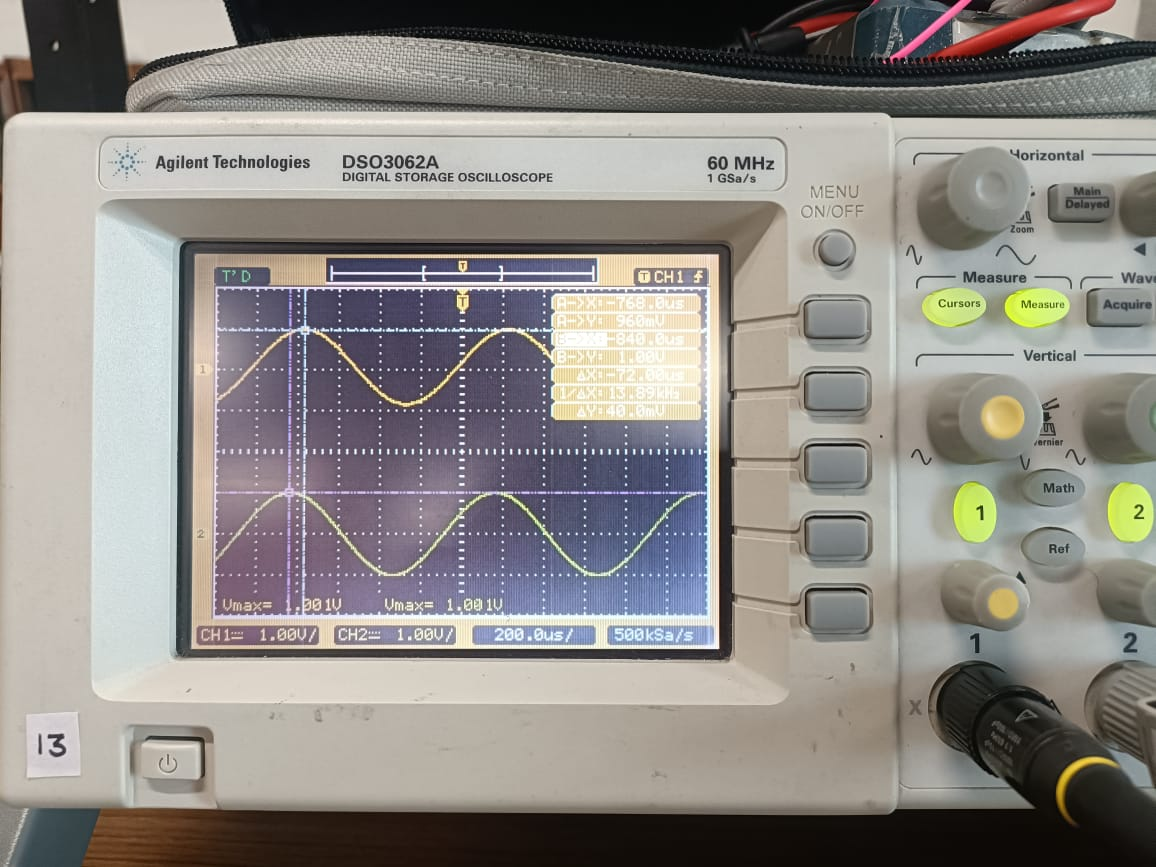
\includegraphics[height=5cm]{figs/Stage1/1000/plot.jpeg}
    \end{subfigure}
\end{figure}
\begin{figure}[H]
    \centering
    \begin{subfigure}{0.5\textwidth}
        \centering
        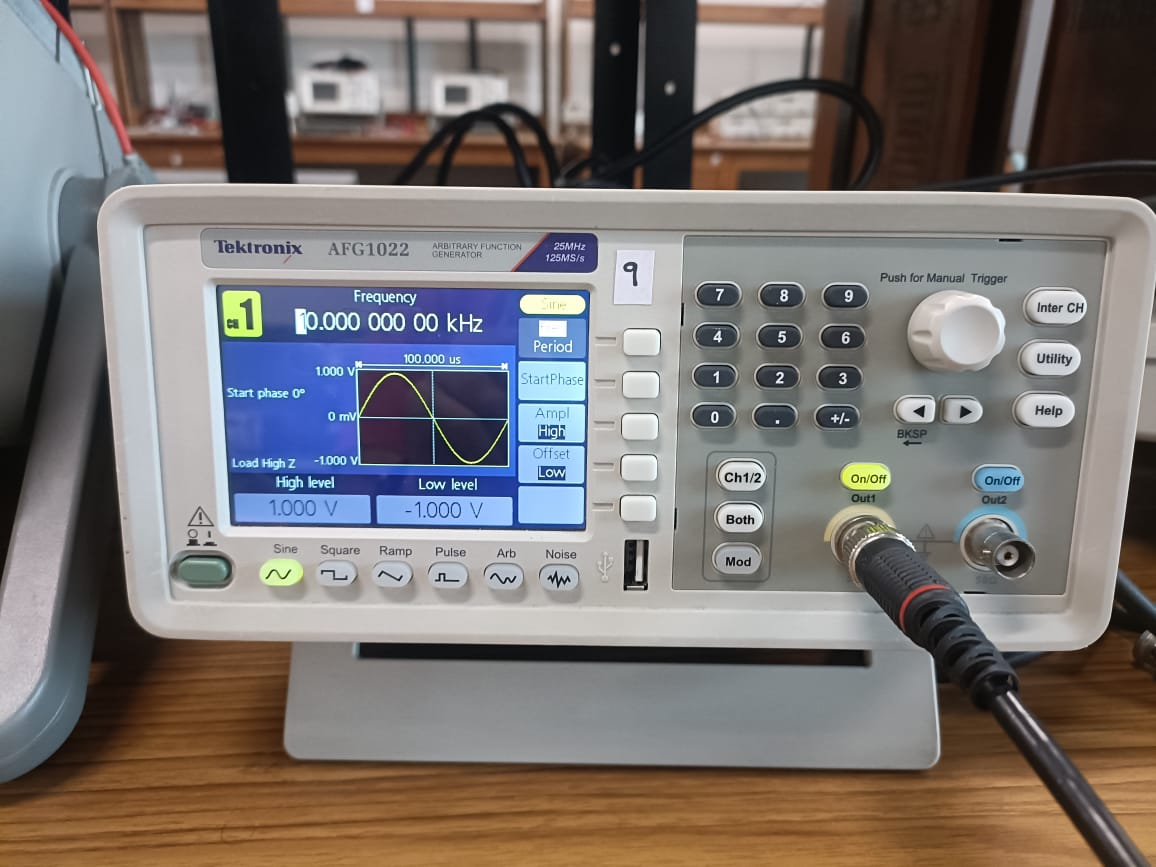
\includegraphics[height=5cm]{figs/Stage1/10000/para.jpeg}
    \end{subfigure}%
    \begin{subfigure}{0.5\textwidth}
        \centering
        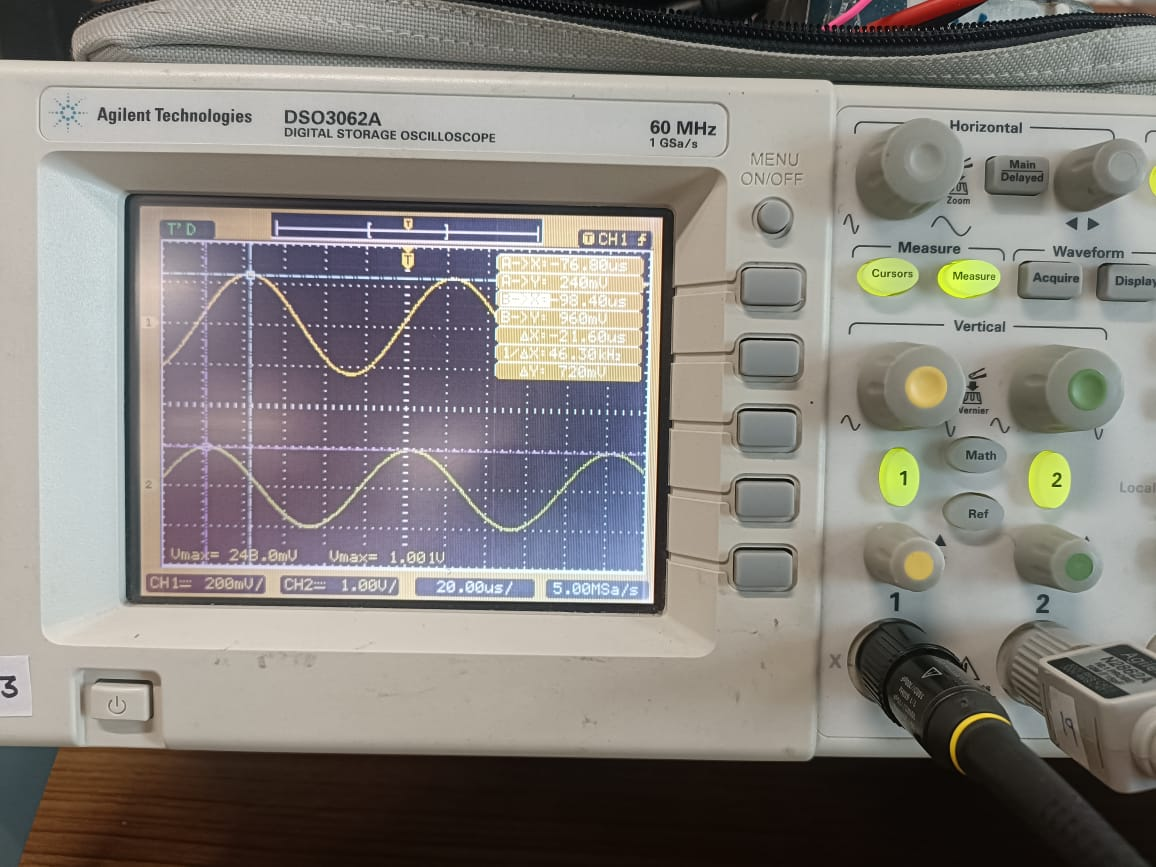
\includegraphics[height=5cm]{figs/Stage1/10000/plot.jpeg}
    \end{subfigure}
\end{figure}
\begin{table}[H]
    \centering
    \begin{tabular}{|c|c|c|}
        \hline
        Frequency (Hz) &  $|H_n(j\omega)|_{dB}$(dB) & Phase (deg) \\
        \hline
        $10^2$ & 0 &-0.3 \\
        $10^3$ & -0.81643989 & -3.0 \\
        $10^4$ & -28.54232711& -30.0 \\
        \hline
    \end{tabular}
    \caption{Stage1}
\end{table}
\subsection*{Stage2}
\begin{figure}[H]
    \centering
    \begin{subfigure}{0.5\textwidth}
        \centering
        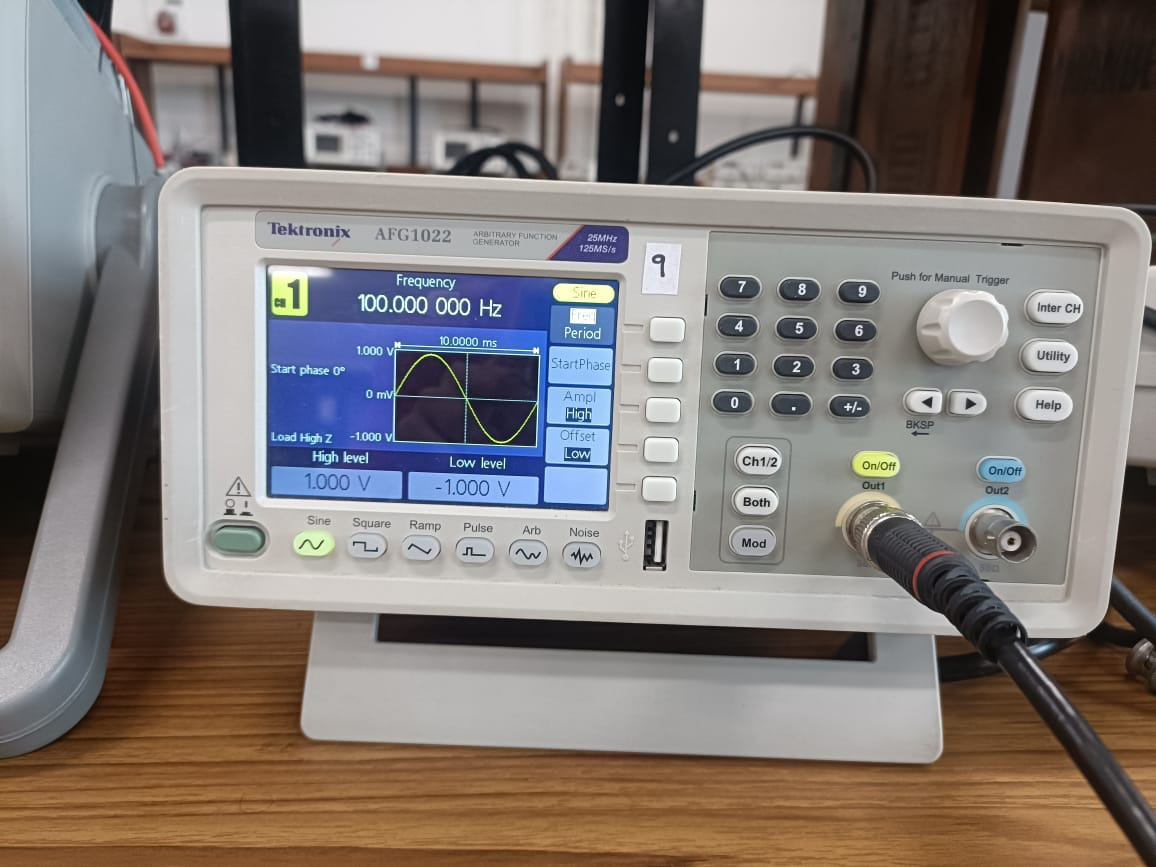
\includegraphics[height=5cm]{figs/Stage2/100/para.jpeg}
    \end{subfigure}%
    \begin{subfigure}{0.5\textwidth}
        \centering
        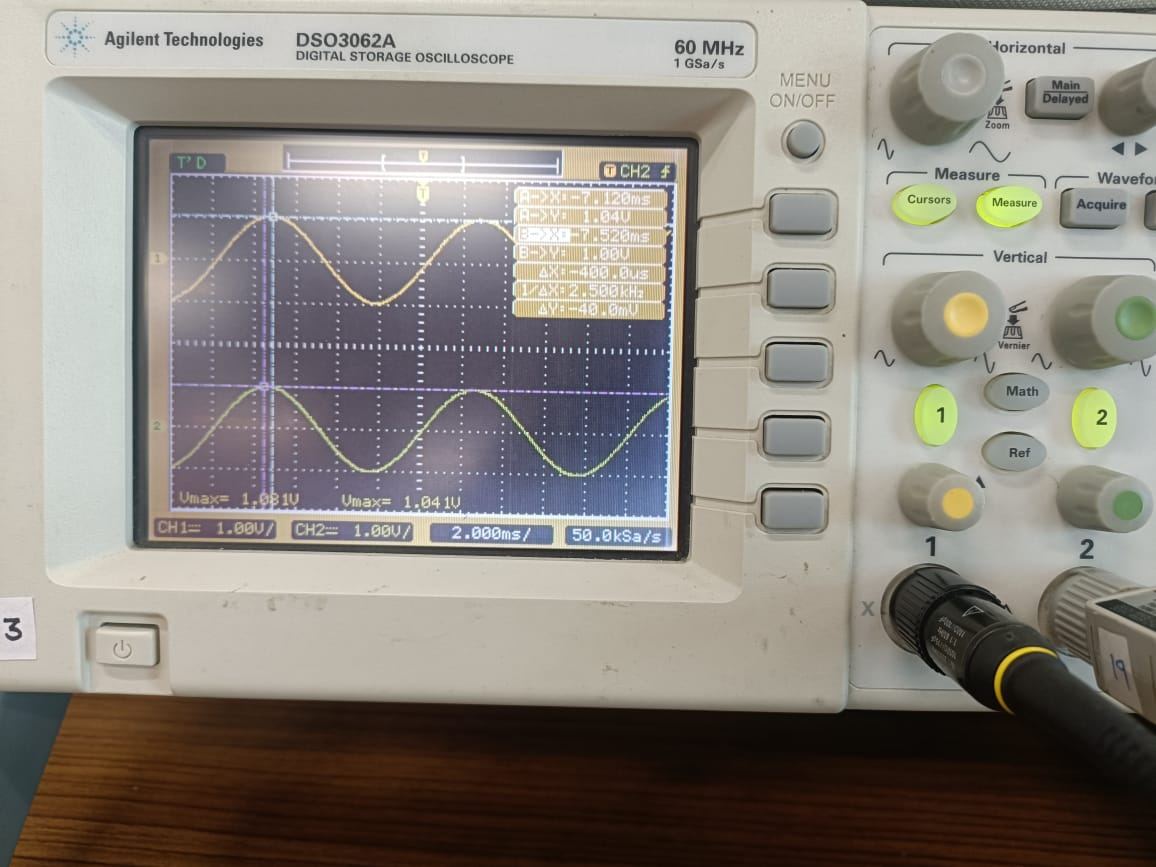
\includegraphics[height=5cm]{figs/Stage2/100/plot.jpeg}
    \end{subfigure}
\end{figure}
\begin{figure}[H]
    \centering
    \begin{subfigure}{0.5\textwidth}
        \centering
        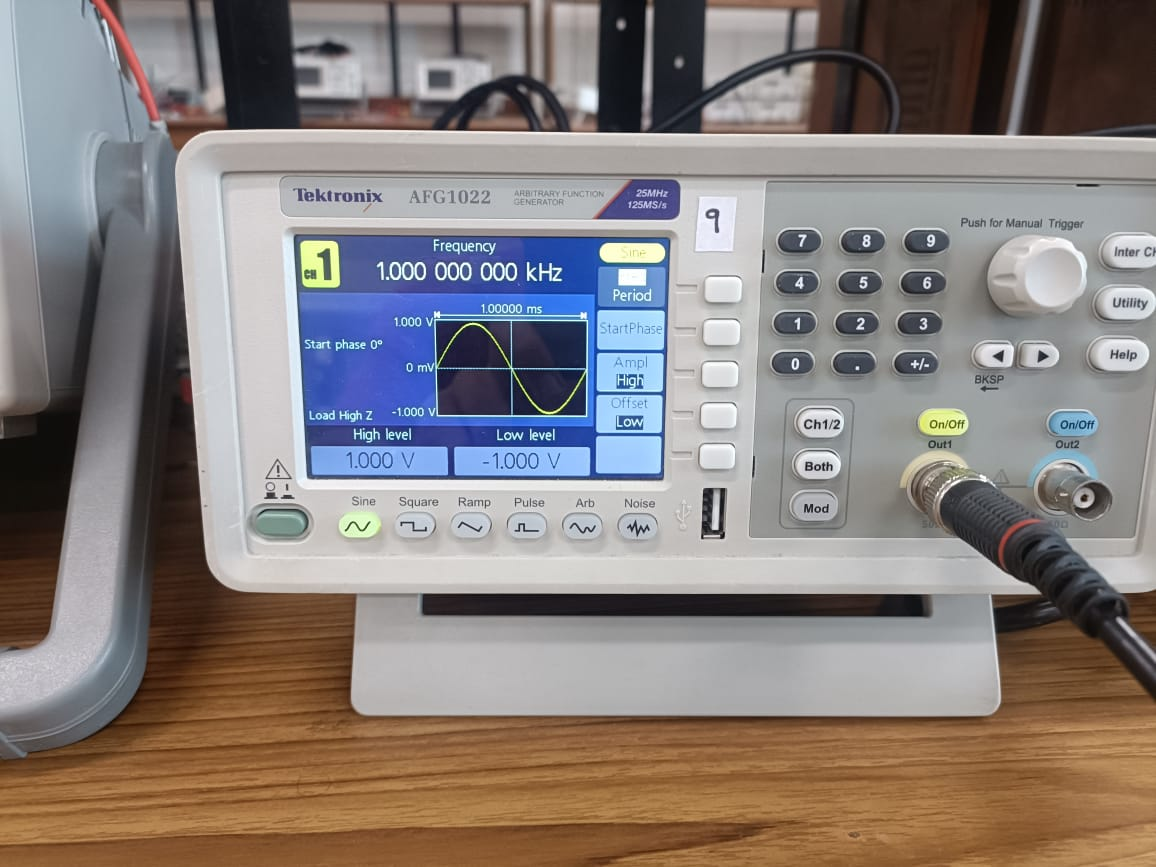
\includegraphics[height=5cm]{figs/Stage2/1000/para.jpeg}
    \end{subfigure}%
    \begin{subfigure}{0.5\textwidth}
        \centering
        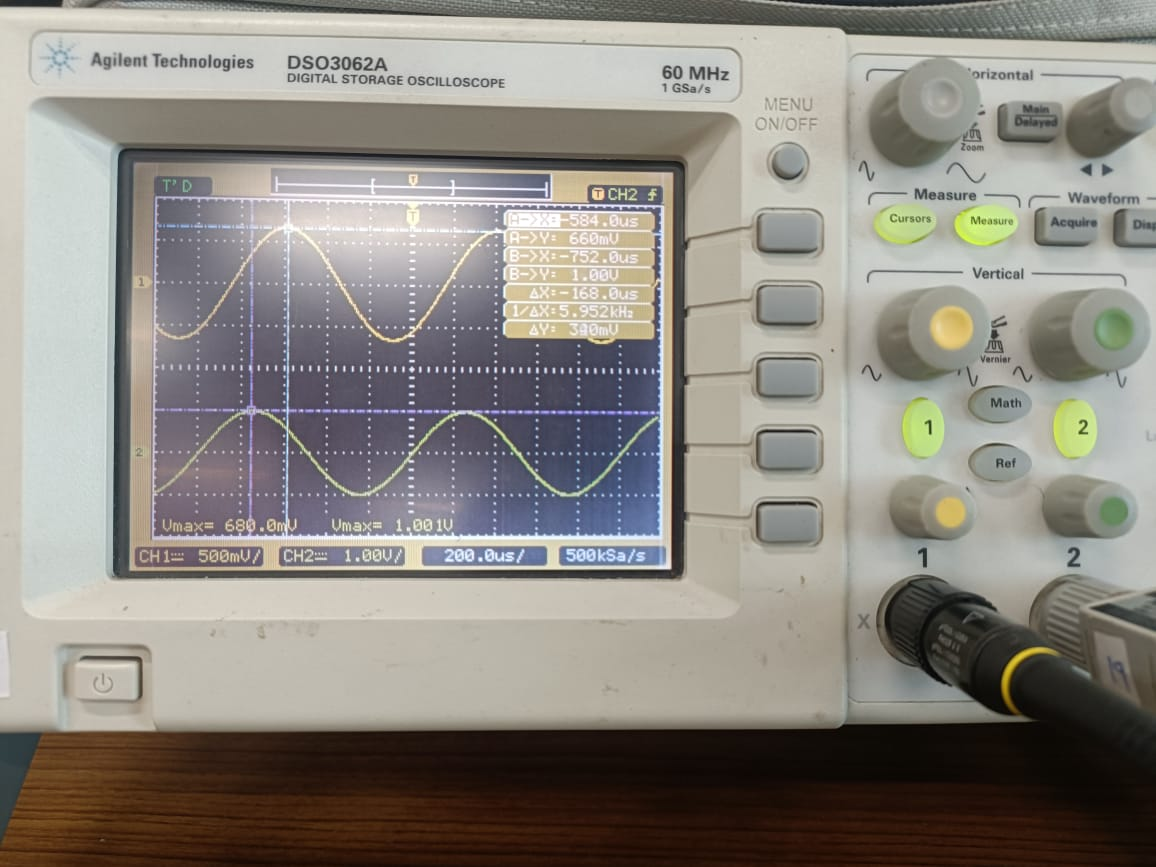
\includegraphics[height=5cm]{figs/Stage2/1000/plot.jpeg}
    \end{subfigure}
\end{figure}
\begin{figure}[H]
    \centering
    \begin{subfigure}{0.5\textwidth}
        \centering
        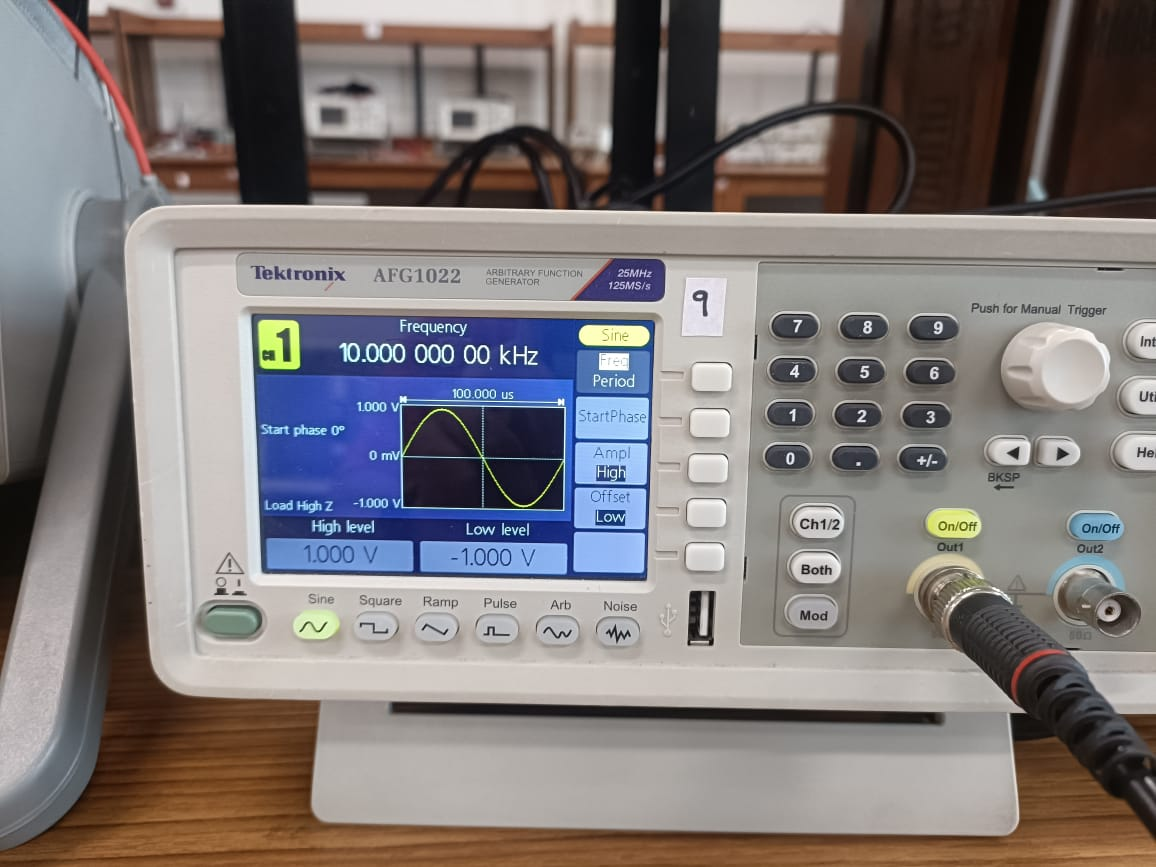
\includegraphics[height=5cm]{figs/Stage2/10000/para.jpeg}
    \end{subfigure}%
    \begin{subfigure}{0.5\textwidth}
        \centering
        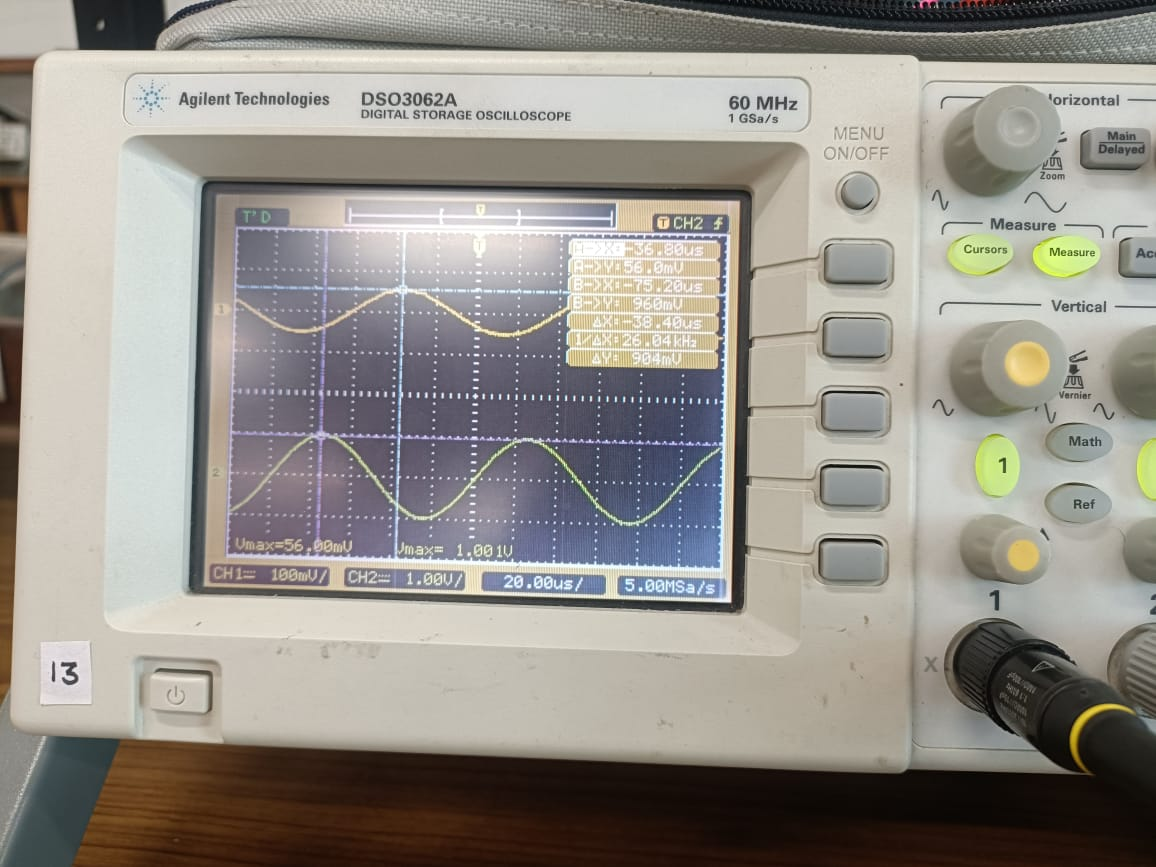
\includegraphics[height=5cm]{figs/Stage2/10000/plot.jpeg}
    \end{subfigure}
\end{figure}
\begin{table}[H]
    \centering
    \begin{tabular}{|c|c|c|c|}
        \hline
        Frequency (Hz) &  $|H_n(j\omega)|_{dB}$(dB) & Phase (deg) \\
        \hline
        $10^2$ & 0 &-14.4 \\
        $10^3$ & -8.31030888 & -60.48 \\
        $10^4$ & -57.64807176& 48.24 \\
        \hline
    \end{tabular}
    \caption{Stage2}

    
\end{table}
\subsection*{Stage3}
\begin{figure}[H]
    \centering
    \begin{subfigure}{0.5\textwidth}
        \centering
        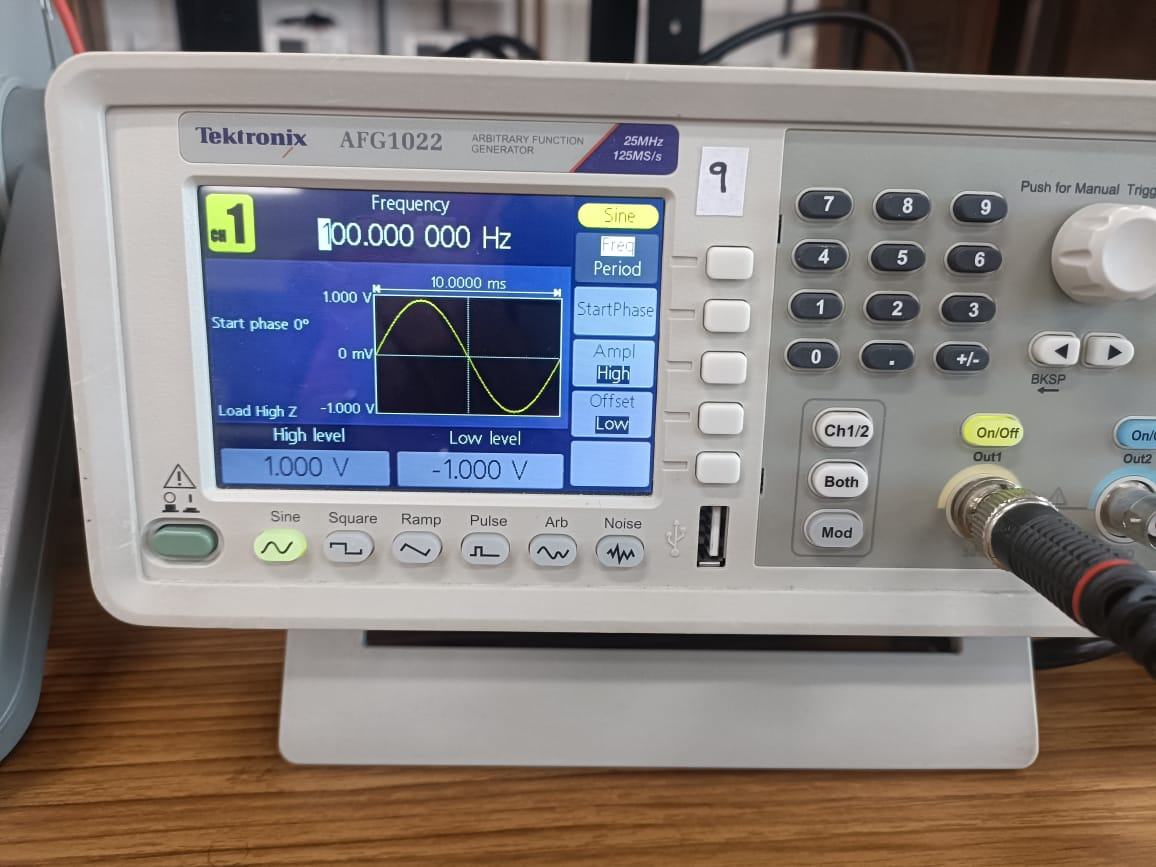
\includegraphics[height=5cm]{figs/Stage3/100/para.jpeg}
    \end{subfigure}%
    \begin{subfigure}{0.5\textwidth}
        \centering
        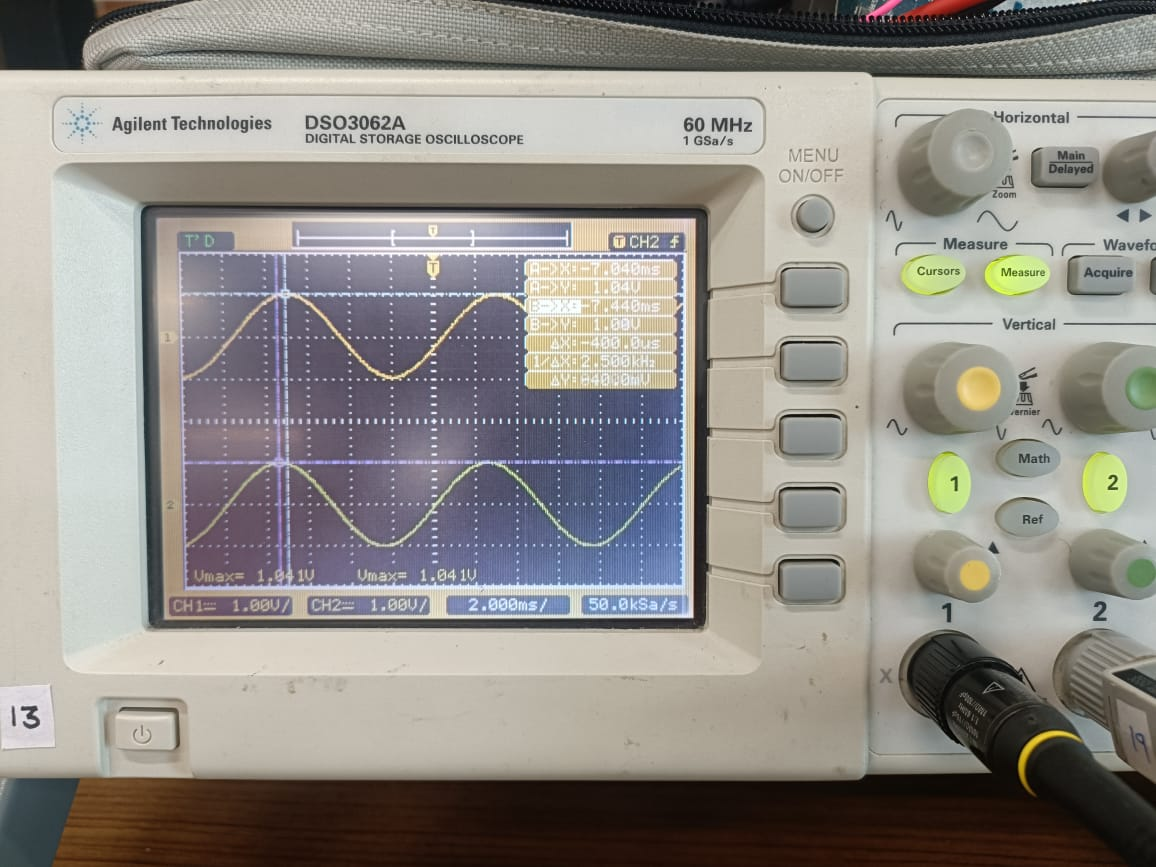
\includegraphics[height=5cm]{figs/Stage3/100/plot.jpeg}
    \end{subfigure}
\end{figure}
\begin{figure}[H]
    \centering
    \begin{subfigure}{0.5\textwidth}
        \centering
        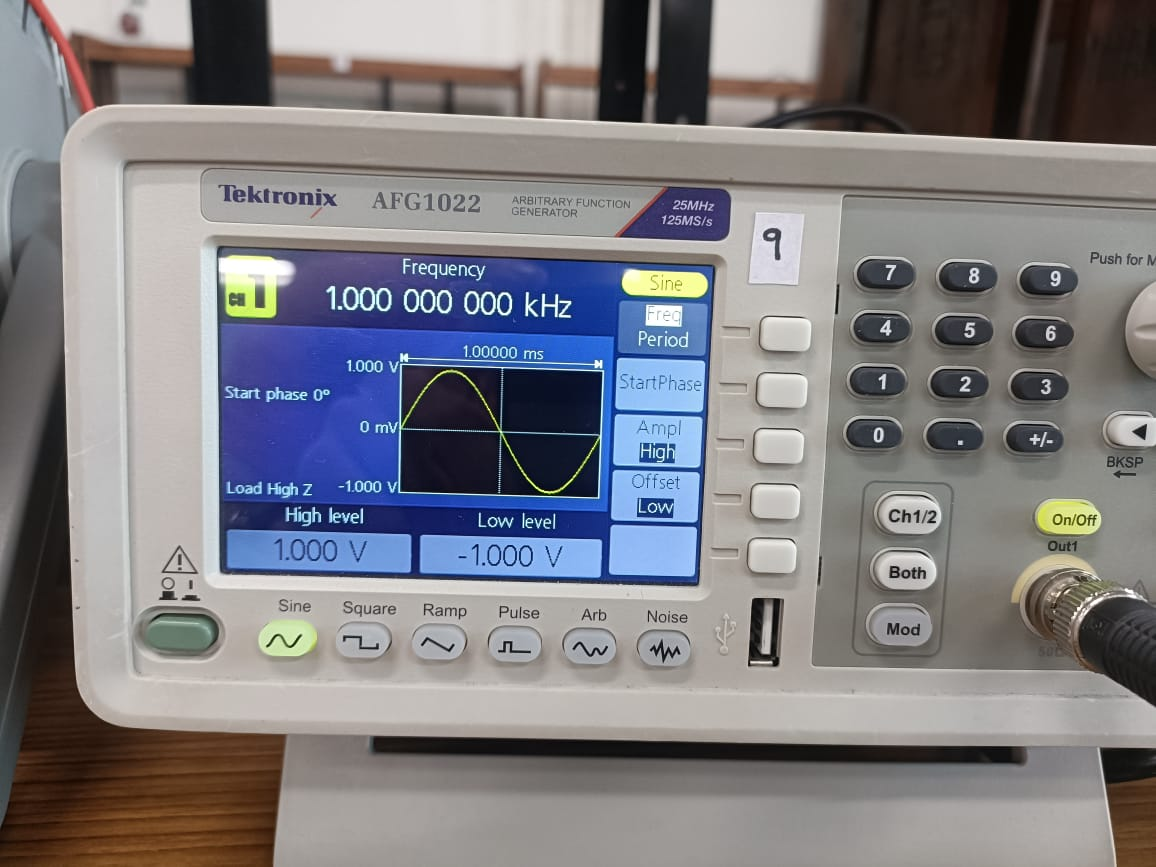
\includegraphics[height=5cm]{figs/Stage3/1000/para.jpeg}
    \end{subfigure}%
    \begin{subfigure}{0.5\textwidth}
        \centering
        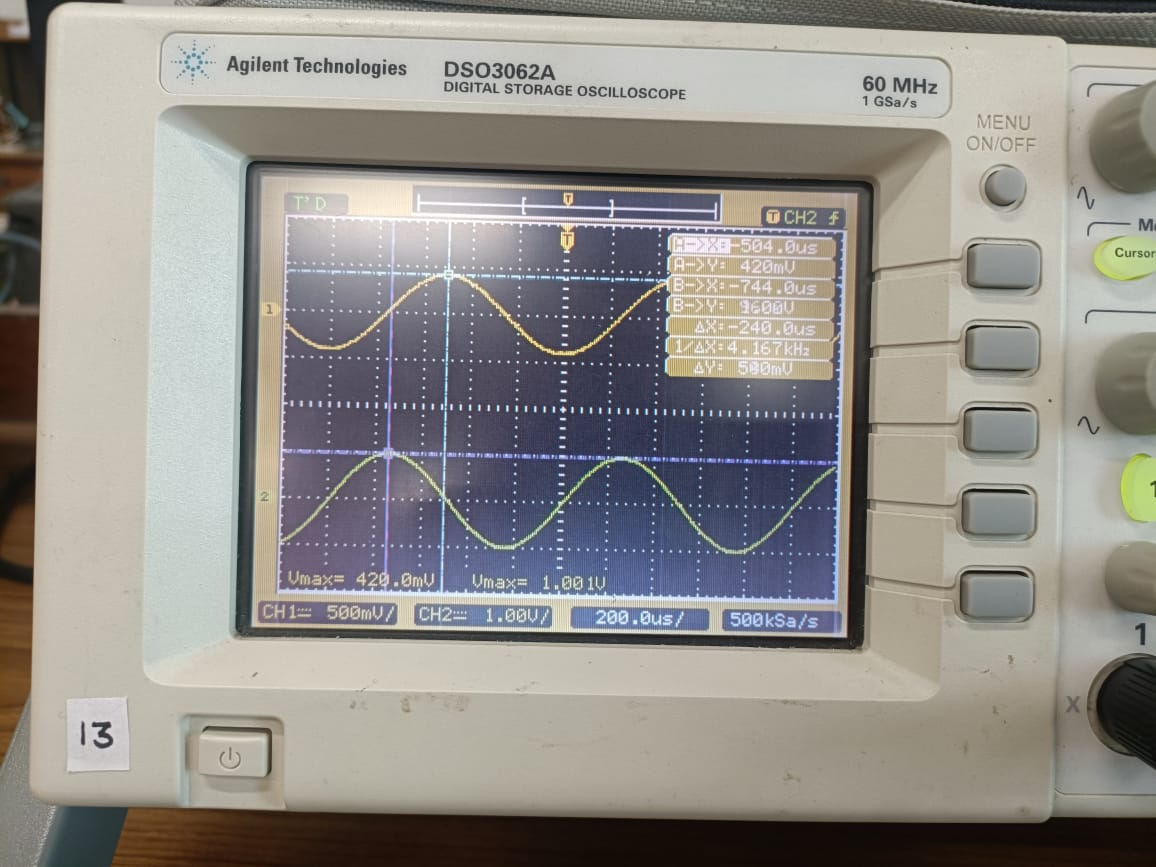
\includegraphics[height=5cm]{figs/Stage3/1000/plot.jpeg}
    \end{subfigure}
\end{figure}
\begin{figure}[H]
    \centering
    \begin{subfigure}{0.5\textwidth}
        \centering
        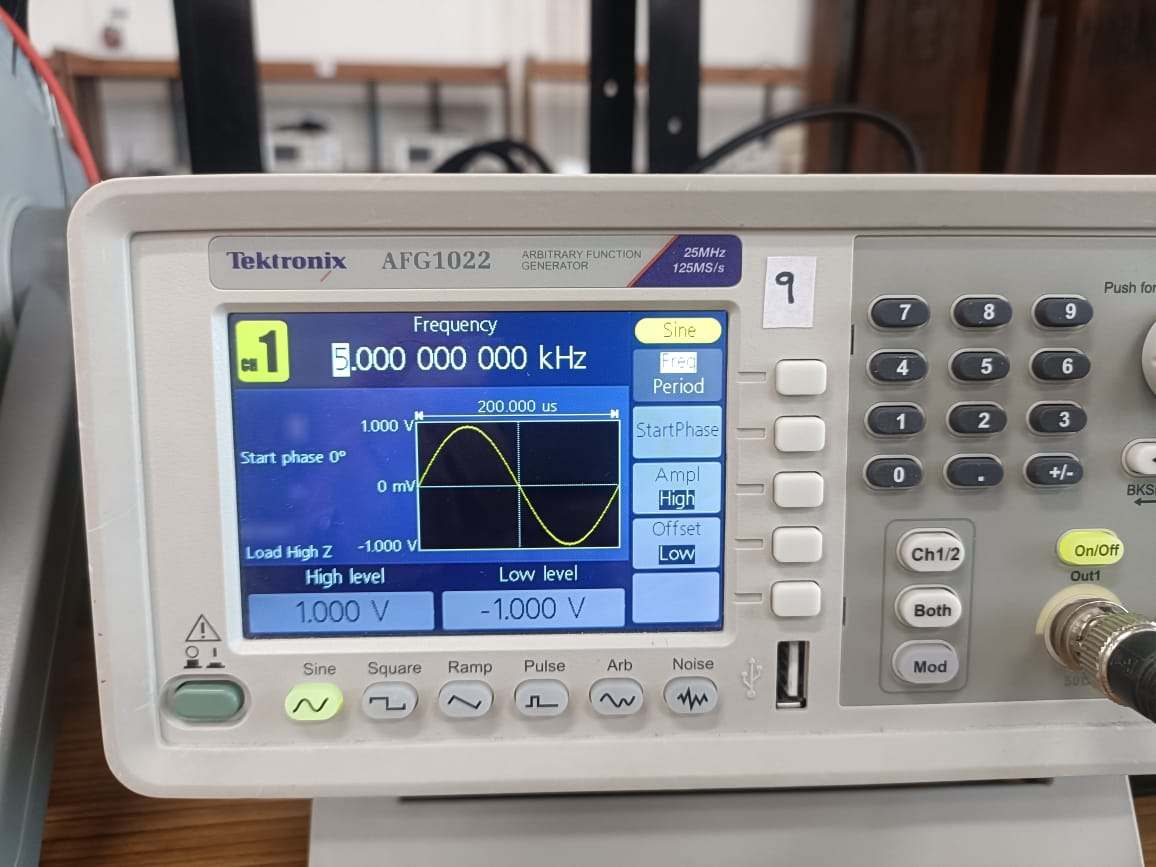
\includegraphics[height=5cm]{figs/Stage3/4000/para.jpeg}
    \end{subfigure}%
    \begin{subfigure}{0.5\textwidth}
        \centering
        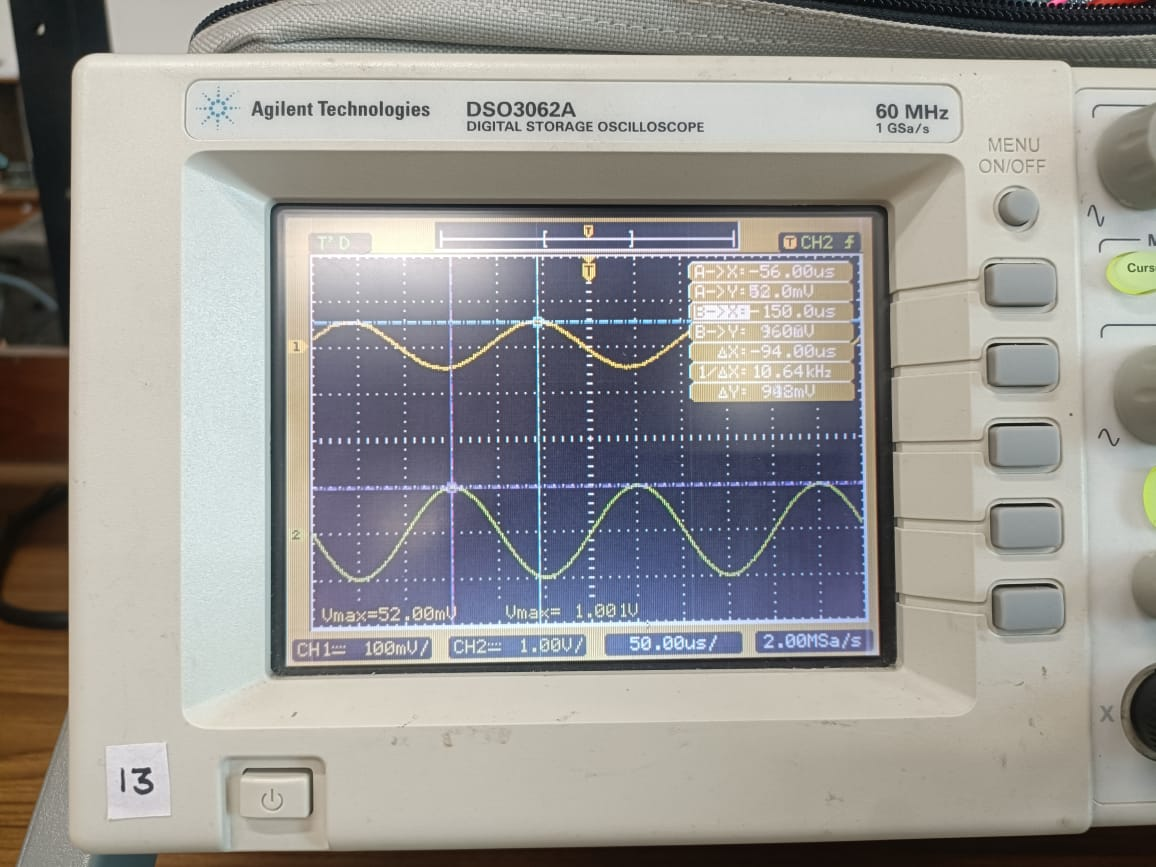
\includegraphics[height=5cm]{figs/Stage3/4000/plot.jpeg}
    \end{subfigure}

    
\end{figure}

\begin{table}[H]
    \centering
    \begin{tabular}{|c|c|c|c|}
        \hline
        Frequency (Hz) &  $|H_n(j\omega)|_{dB}$(dB) & Phase (deg) \\
        \hline
        $10^2$ & 0 &-14.4 \\
        $10^3$ & -17.35001135 & -86.4 \\
        $10^4$ & -59.13023121& -79.2 \\
        \hline
    \end{tabular}
    \caption{Stage3}
\end{table}

\section*{Graphs}
\subsection*{Stage1}
\begin{figure}[H]
    \centering
    \begin{subfigure}{0.5\textwidth}
        \centering
        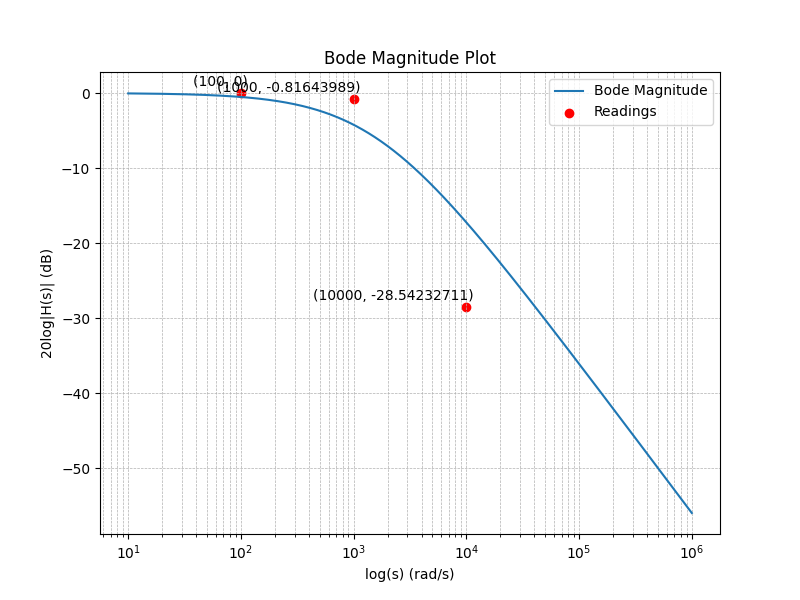
\includegraphics[height=5cm]{figs/Stage1/Magn.png}
    \end{subfigure}%
    \begin{subfigure}{0.5\textwidth}
        \centering
        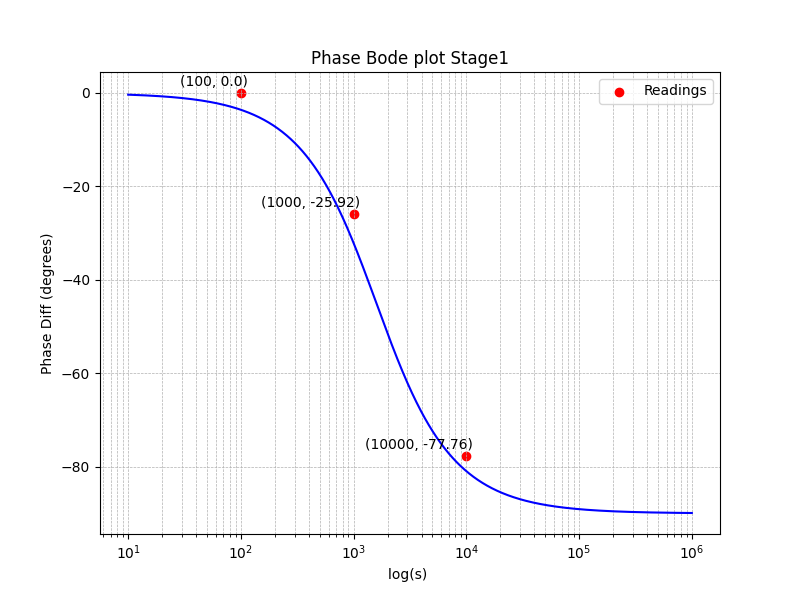
\includegraphics[height=5cm]{figs/Stage1/Phase.png}
    \end{subfigure}
\end{figure}

\subsection*{Stage2}
\begin{figure}[H]
    \centering
    \begin{subfigure}{0.5\textwidth}
        \centering
        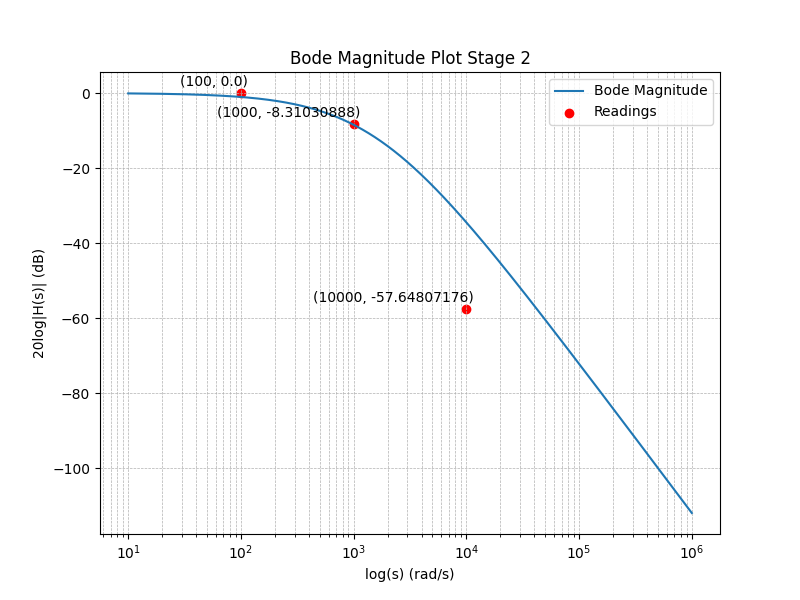
\includegraphics[height=5cm]{figs/Stage2/Magn.png}
    \end{subfigure}%
    \begin{subfigure}{0.5\textwidth}
        \centering
        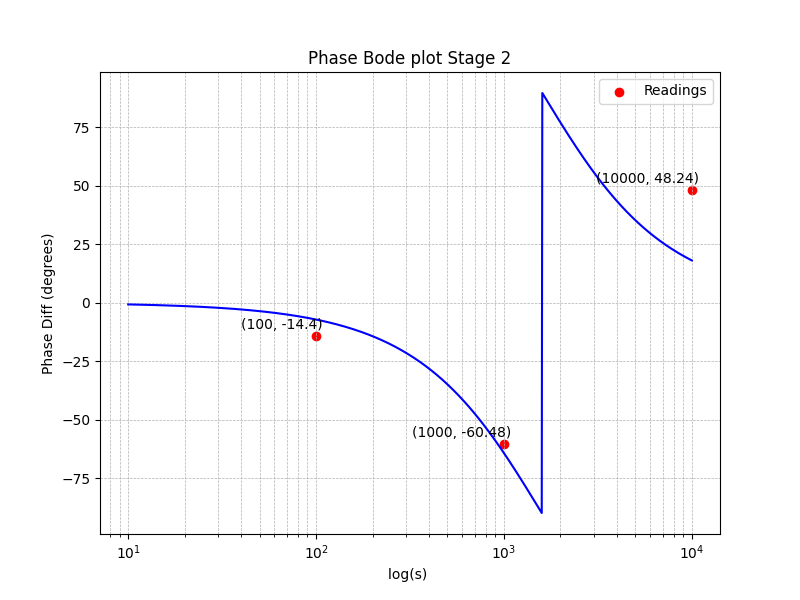
\includegraphics[height=5cm]{figs/Stage2/Phase.png}
    \end{subfigure}
\end{figure}

\subsection*{Stage3}
\begin{figure}[H]
    \centering
    \begin{subfigure}{0.5\textwidth}
        \centering
        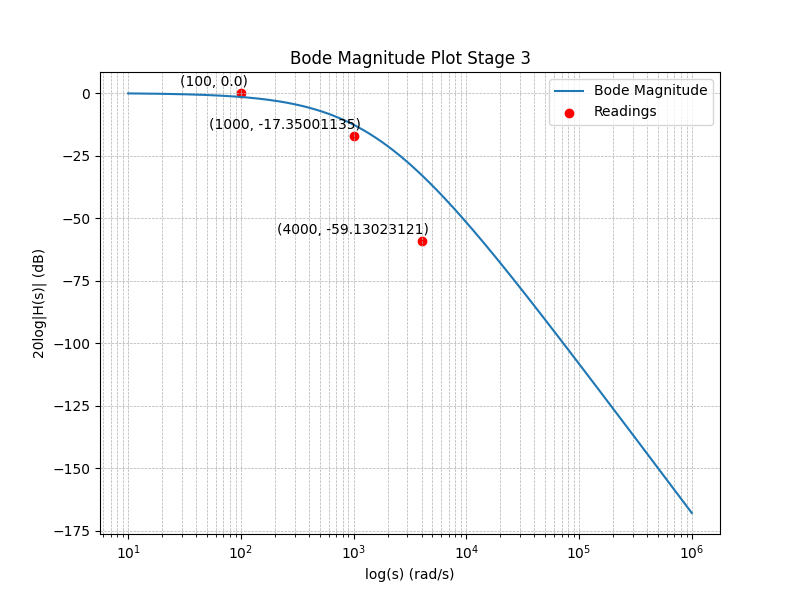
\includegraphics[height=5cm]{figs/Stage3/Magn.png}
    \end{subfigure}%
    \begin{subfigure}{0.5\textwidth}
        \centering
        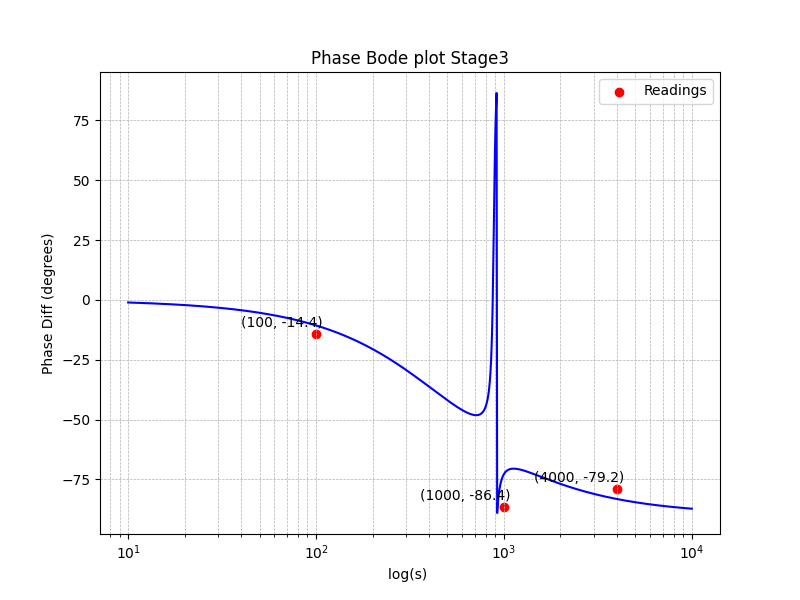
\includegraphics[height=5cm]{figs/Stage3/Phase.png}
    \end{subfigure}
\end{figure}
\centering{Thank You}
\end{document}

